\documentclass[12pt]{article}

\usepackage{amssymb,amsmath}
\usepackage[margin=1.0in]{geometry}
\usepackage{fancyhdr} % required for custom header
\usepackage{graphicx}
\usepackage{listings}
\usepackage{courier}
\usepackage[usenames,dvipsnames]{color}

%set up the header
\pagestyle{fancy}
\lhead{Trever Hines}
\chead{El Mayor Postseismic}
\rhead{\today}

\setlength{\headheight}{15pt}
\renewcommand\headrulewidth{1.0pt} % Size of the header rule

%% Title
%%------------------------------------------------------------------------------
\title{	
El Mayor Postseismic
\author{Trever Hines}
\rule{\headwidth}{1.0pt}
}

\begin{document}
\maketitle
\section*{Introduction}

Previous studies which have modeled postseismic deformation following the El Mayor-Cucapah earthquake include \cite{Pollitz2012}, \cite{Gonzalez-ortega2014}, \cite{Spinler2015}, and \cite{Rollins2015}. \cite{Gonzalez-ortega2014} was able to describe five months of near field ($\lesssim 50$ km from the epicenter) postseismic defomation observed by InSAR and campaign GPS with afterslip and fault contraction on the coseismically ruptured fault. \cite{Gonzalez-ortega2014} also noted that their preferred model underestimated the GPS displacements for stations $\gtrsim 25$ km from the rupture and suggested that it could be the result of unmodeled viscoelastic relaxation.  Using continuous GPS stations within 200 km of the El Mayor-Cucapah epicent, which consists mostly of stations north of the US-Mexico border, \cite{Rollins2015} found that three years of postseismic deformation can be adequately explained by afterslip in an elastic lithosphere, albeit with an implausibly large amount of afterslip inferred on the least constrained southern most fault segment which may be acting as a proxy for distributed relaxation in the lower crust or upper mantle. In this paper, we reiterate this finding by \cite{Rollins2015} and note that a purely elastic dislocation model is incapable of describing deformation observed at GPS stations greater than ~200 km from the El Mayor-Cucapah epicenter.  

Given the inability to describe both near and far field deformation with fault slip in an elastic lithosphere, \cite{Pollitz2012}, \cite{Rollins2015} and \cite{Spinler2015} have explored viscoelastic relaxation in the lower crust and upper mantle as a potential deformation mechanism. The lithospheric rheology is largely unknown and so modeling postseismic deformation with viscoelastic relaxation requires one to assume a rheologic model and find the best fitting model parameters, which is generally a computationally expensive nonlinear inverse problem. Consequently, a simplified structure for the lithosphere must be made to minimize the number of rheologic parameters that need to be estimated.  For example, it is commonly assumed that the lithosphere consists of only three homogeneously Maxwell viscoelastic layers, which may be an inadequate representation of the lithosphere \cite{Hines2013}\cite{Riva2009}. Additionally, it is necessary to make simplifying assumptions about the nature of afterslip. For example, one can assume a frictional model for afterslip and parameterize afterslip in terms its the unkown rheologic properties (e.g. \cite{Johnson2009} \cite{Johnson2004}). Additionally, one can assume that afterslip only dominates the first year of deformation (e.g. \cite{Pollitz2012} and \cite{Spinler2015}) and that viscoelastic relaxation is the dominant mechanism in later years. However, numerous observations of interseismic fault creep has been recognized in this and similar tectonic settings and it has been speculated that such creep can be initiated as a postseismic process \cite{Cakir2012} \cite{Cetin2014}.  We are unaware of any oIn this study, we therefore do not make to implicit assumption that afterslip terminates after a given amount of time.  Indeed, the preferred viscoelastic model from \cite{Pollitz2012} underpredicts near field velocities, which could be indicative of unmodeled continued afterslip.

All of the aforementioned studies model displacements observered at stations within 200 km of the El Mayor-Cucapah epicenter, while postseismic deformation in this region following previous earthquakes of similar magnitude has been observed at distances extended out to about 300 km \cite{Freed2007a}. In the present study we examine stations within 400 km of the El Mayor-Cucapah epicenter, which turns out to be crucial for discerning the postseismic deformation mechanism.

Clearly, both afterslip and viscoelastic relaxation are involved in postseismic deformation neglecting to model one of these deformation mechanisms could result in a biased estimate of the other.  In this paper we use the inverse method described in \cite{Hines2015} to estimate the afterslip an effective viscosity necessary to describe the transience postseismic deformation over the first ten months after the El Mayor-Cucapah earthquake. We then form a suite of models which have various lithospheric rheologies but viscosities that are consistent with the effective viscosity estimated from the early postseismic deformation. Of the suite of models tested, we find that five years of postseismic deformation can be explained by a combination of sustained afterslip on the coseismicly ruptured fault and a Zener rheology upper mantle with viscosity that decays from $4\times10^{18}$ to $1\times10^{18}$ Pa s. 


\section*{Data Processing}

We use continuous GPS position time series provided by University Navstar Consortium (UNAVCO) for Plate Boundary Observatory (PBO) stations within a 400 km radius about the El Mayor-Cucapah epicenter. Our analysis is on the coseismic and postseismic deformation resulting from the EMC earthquake, which we collectively describe as $u(t)$. We consider GPS position time series, $u_\mathrm{obs}(t)$, to be the superposition of $u(t)$, secular tectonic deformation, annual and semi-annual fluctuations, and coseismic offsets from sigificant earthquakes over the time span of this study.  The June 14, 2010 Mw5.8 Ocotillo earthquake and the August 26, 2012 Brawley swarm, which consisted of a Mw5.5 and Mw5.3 event, are the only earthquakes after the EMC earthquake that produced noticeable offsets recorded by GPS. Although the Ocotillo earthquake had its own series of aftershocks (Haukson), neither earthquake produced transient deformation that is detectable with GPS. We thus model $u_\mathrm{obs}(t)$ as 

\begin{equation}
  u_\mathrm{obs}(t) = u_\mathrm{pred}(t) + \epsilon
\end{equation}
where
\begin{equation}\label{TimeSeriesModel}
  \begin{split}  
    u_\mathrm{pred}(t) = &u(t) + c_0 + c_1t + \\
                         &c_2\sin(2\pi t) + c_3\cos(2\pi t) + c_4\sin(4\pi t) + c_5\cos(4\pi t) + \\
                         &c_6H(t-t_\mathrm{oc}) + c_7H(t-t_\mathrm{bs}).
  \end{split}
\end{equation}
In the above equations, $t_\mathrm{oc}$ and $t_\mathrm{bs}$ are the times of the Ocotillo earthquake and Brawley swarm respectively, $H(t)$ is the Heaviside function, $c_0$ through $c_7$ are unknown coefficients, and $\epsilon$ is noise with zero mean and variance that assumed known.

Stations which recorded signals that clearly cannot be described by the aforementioned processes are not included in our analysis. This includes stations in the Los Angeles basin, which record deformation that is largely anthropogenic. In order to ensure an accurate estimation of the secular deformation, we only use stations that were installed at least six months prior to El Mayor-Cucapah earthquake. While several stations were installed after the EMC earthquake to improve the spatial resolution of postseismic deformation \cite{Spinler2015}, our inverse method uses postseismic displacements rather than velocities (e.g. ...), which requires the knowledge of the stations preseismic position. Despite our inability to utilize potentially rich data, we prefer to use postseismic displacements rather than potentially dubious estimates of postseismic velocities.

The October 16, 1999 Hector Mine earthquake, which occurred within our study region about 270 km north of the EMC epicenter, has produce transient postseismic deformation which we do not wish to model either mechanically or through empirical line fitting. We thus restrict our analysis to deformation observed six years after the Hector Mine earthquake, past which point postseismic deformation for nearfield sites occurs at an approximately steady rate \cite{Savage2009}. When considering stations further away from the Hector Mine epicenter, postseismic transience persists for only about two years \cite{Spinler2015}.

Studies of postseismic deformation typically assume a parametric form for $u(t)$ such as such as a logarithmic or exponential function. Such functions have been found empirically e.g. \cite{Savage2005a} and theoretically \cite{Marone1991} to adequately describe deformation resulting from postseismic deformation. However, by assuming a logarithmic or exponential form of $u(t)$ we run the risk of overfitting the GPS time series and inferring a nonexistent postseismic signal. We therefore do not assume any parameteric form for $u(t)$ and rather treat it as integrated Brownian motion, so that 
\begin{equation}
    \dot{u}(t) = \sigma^2\int_0^t w(s) ds.
\end{equation}    

where $w(t)$ is white noise and the variance of $\dot{u}(t)$ increases linearly with time by a factor of $\sigma^2$. We use a
Kalman filtering approach to estimate $u(t)$ and the unknown parameters in eq. \ref{TimeSeriesModel} which we describe now.  In the context of Kalman filtering, our time varying state vector is
\begin{equation}
    \mathbf{X}(t) = [u(t),\dot u(t), c_0, ..., c_7]
\end{equation}
and eq. \ref{TimeSeriesModel} is the observation function which maps the state vector to the GPS observations. We initiate the Kalman filter by assuming a prior estimate of $\mathbf{X}(t)$ at time $t_0$ which has a sufficiently large covariance to effectively make our prior uninformed.  For each time epoch, $t_i$, Bayesian linear regression is used to incorperate GPS derived estimates of displacement with our prior estimate of the state, $\mathbf{X}_{i|i-1}$, to form a postserior estimate of the state, $\mathbf{X}_{i|i}$, which has covariance $\mathbf{\Sigma}_{i|i}$.  

We then use the posterior estimate of the state at time $t_i$ to form a prior estimate of the state at time $t_{i+1}$ through the transition function
\begin{equation}\label{predict}
  \mathbf{X}_{i+1|i} = \mathbf{F}_{i+1}\mathbf{X}_{i|i} + \mathbf{\delta}_{i+1} 
\end{equation}
where 
\begin{equation}
  \mathbf{F}_{i+1} = 
  \left[
  \begin{array}{ccc}
    1           & (t_{i+1} - t_i) & \mathbf{0}\\
    0           & 1              & \mathbf{0}\\
    \mathbf{0}  & \mathbf{0}     & \mathbf{I}
  \end{array}
  \right]
\end{equation}
and $\mathbf{\delta}_{i+1}$ is the process noise, which has zero mean and covariance described by
\begin{equation}
  \mathbf{Q}_{i+1} = 
  \sigma^2 \left[
  \begin{array}{ccc}
  \frac{(t_{i+1} - t_i)^3}{3} & \frac{(t_{i+1} - t_{i})^2}{2} & \mathbf{0}\\
  \frac{(t_{i+1} - t_i)^2}{2} & (t_{i+1} - t_{i}) & \mathbf{0}\\ 
  \mathbf{0} & \mathbf{0} & \mathbf{0}
  \end{array}
  \right].
\end{equation}

The covariance of the new prior state, $\mathbf{X}_{i+1|i}$, is then described by
\begin{equation}
  \mathbf{\Sigma}_{i+1|i} = \mathbf{F}_{i+1}\mathbf{\Sigma}_{i|i}\mathbf{F}^T_{i+1} + \mathbf{Q}_{i+1}.
\end{equation}

This process is repeated for each of the $N$ time epochs at which point we use Rauch-Tung-Striebel smoothing to find $X_{i|N}$, which is an estimate of the state at time $t_i$ that incorporates all $N$ GPS observation.  Our final estimates of $u(t)$ are used in subsequent analysis, while the remaining components of of the state vector are considered nuisance parameters. In the interests of computational tractability, we down sample our smoothed time series from daily solutions down to weekly solutions.


\begin{figure}
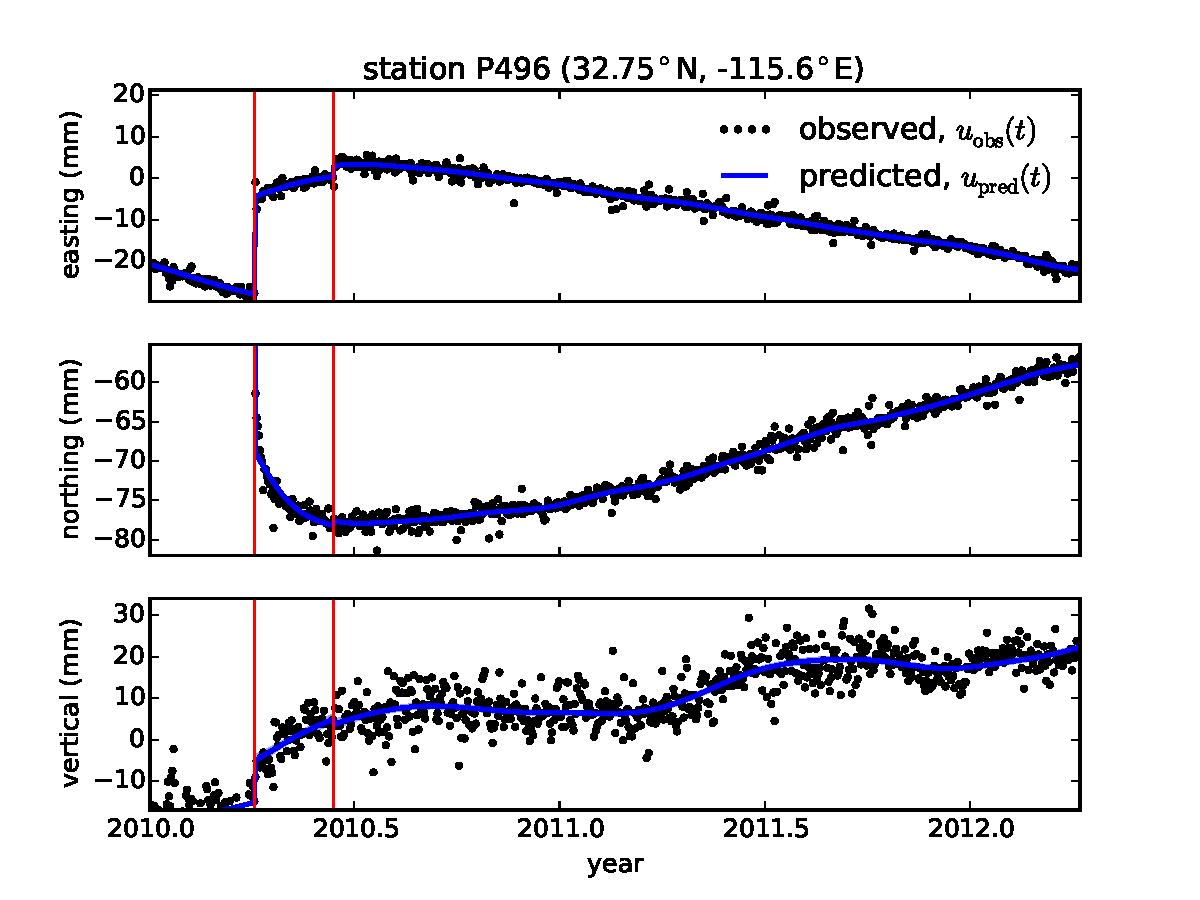
\includegraphics[scale=0.6]{Figures/figure_1}
\centering
\caption{GPS displacement solution from UNAVCO (black) and predicted displacements after applying a Kalman filter where $\sigma^2=0.05 \mathrm{m}^2/\mathrm{yr}^3$. Red line indicates the time of the Ocotillo earthquake where a jump in the time series is estimated}
\label{P496Fit}
\end{figure}

\begin{figure}
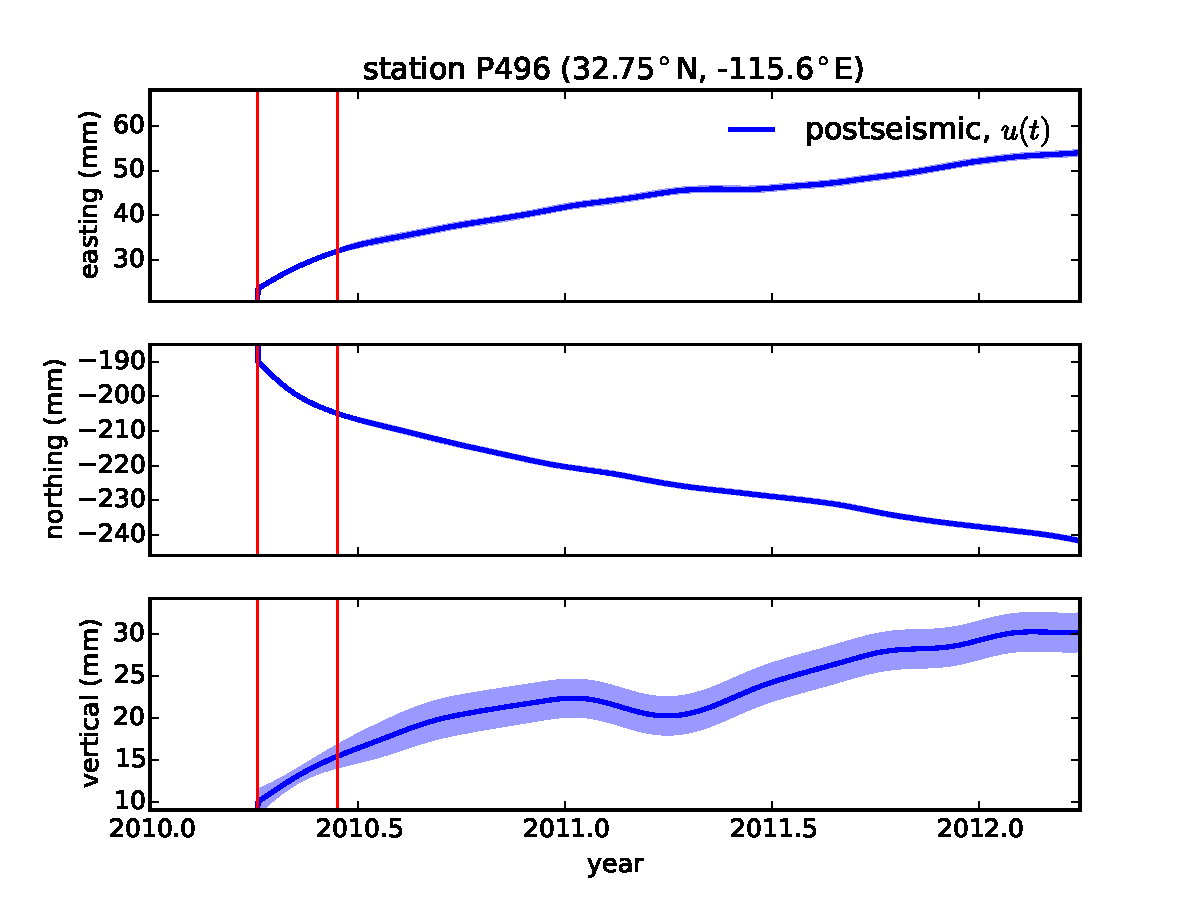
\includegraphics[scale=0.6]{Figures/figure_2}
\centering
\caption{Postseismic displacements estimated after applying a Kalman filter to the GPS displacement solution from UNAVCO.  Displacements shown have had a background secular trend removed as well as an estimated seasonal signal.} 
\label{P496PS}
\end{figure}

\begin{figure}
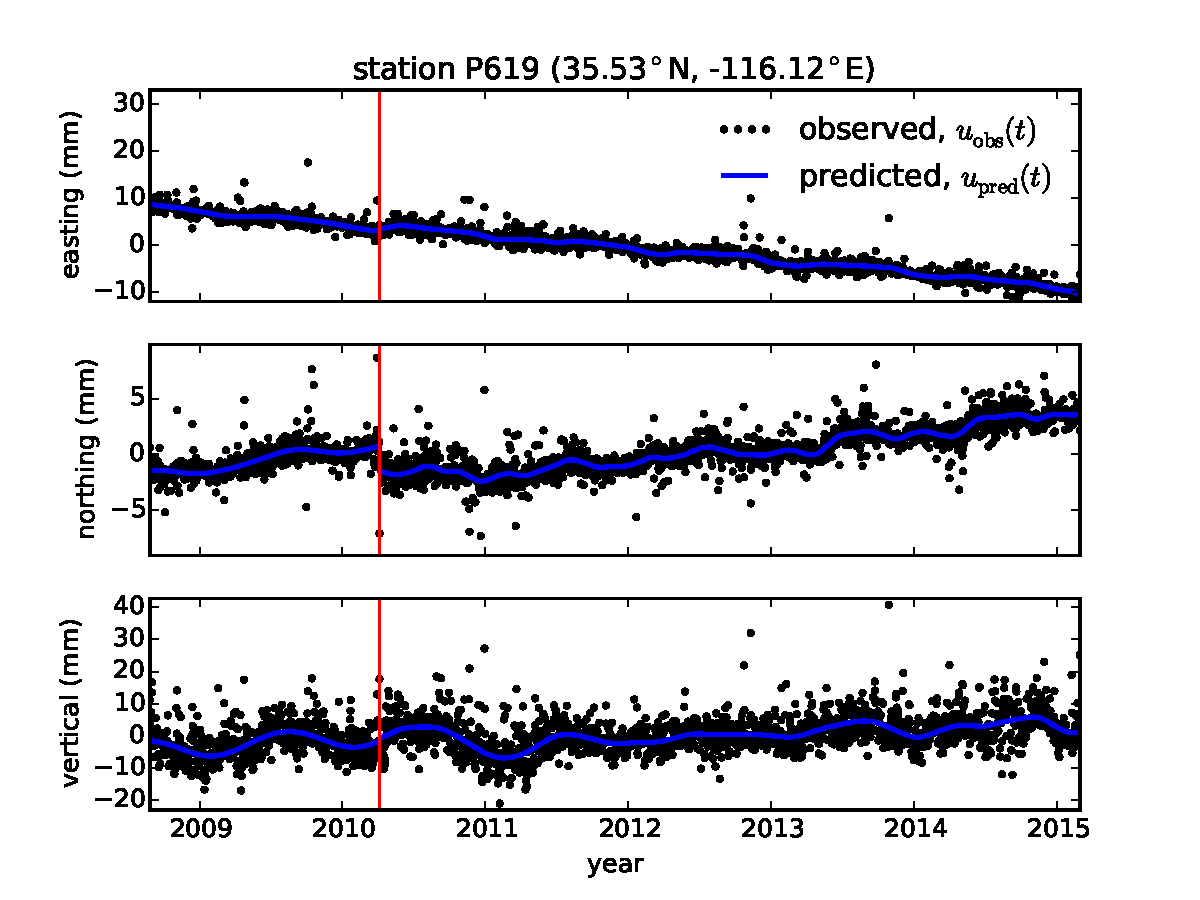
\includegraphics[scale=0.6]{Figures/figure_3}
\centering
\caption{GPS displacement solution from UNAVCO (black) and predicted displacements after applying a Kalman filter where $\sigma^2=0.05 \mathrm{m}^2/\mathrm{yr}^3$. Red line indicates the time of the Ocotillo earthquake where a jump in the time series is estimated}
\label{P619Fit}
\end{figure}

\begin{figure}

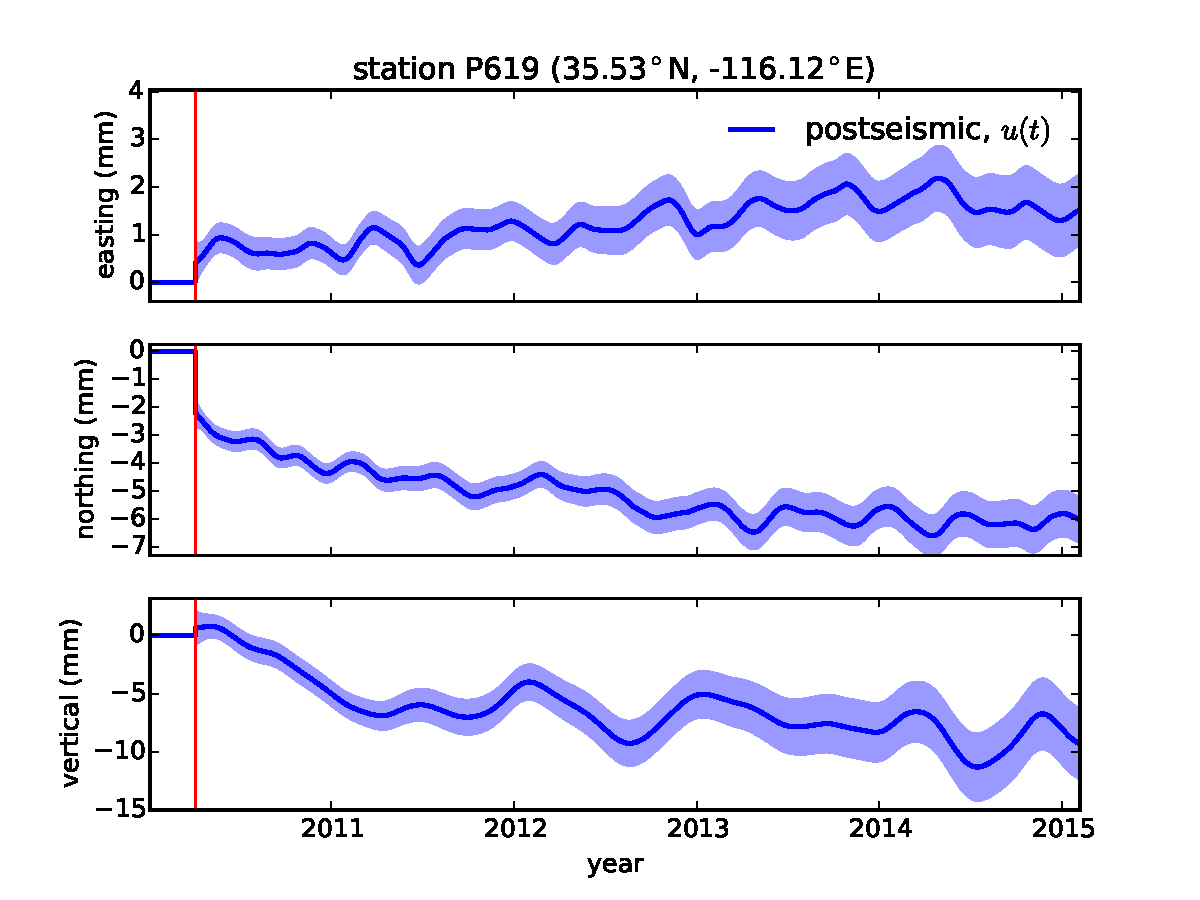
\includegraphics[scale=0.6]{Figures/figure_4}
\centering
\caption{Postseismic displacements estimated after applying a Kalman filter to the GPS displacement solution from UNAVCO.  Displacements shown do not include the estimated secular trend, seasonal signals, and displacements resulting from the Ocotillo earthquake.} 
\label{P619PS}
\end{figure}

The smoothness of $u(t)$ is controlled by the chosen value of $\sigma^2$, which describes how rapidly we expect the postseismic signal to vary over time.  Setting $\sigma^2$ equal to zero will effectively result in modeling $u(t)$ as a straight line which is insufficient to describe the expected transient behavior in postseismic deformation \cite{Savage2005a}. The other endmember, where $\sigma^2$ is infinitely large, will result in $u_\mathrm{pred}(t)$ fitting what is obviously noise in the data. While one can use a maximum likelihood based approach to picking $\sigma^2$ (e.g. \cite{Segall1997}), we rather take a subjective approach and choose a value for $\sigma^2$, which is used when filtering time series for each station, that is just large enough to faithfully describes the early rapid rate of postseismic deformation at the most near field station in our study, P496.  This ensures that $\sigma^2$ will be sufficiently large so that our estimate of $u(t)$ does not smooth out potentially valuable postseismic signal. We find that when using $\sigma^2 = 0.05 \mathrm{m}^2 / \mathrm{yr}^3$, we are able to adequately describe all but the first week of postseismic deformation at station P496, which gets incorporated into our estimate of coseismic displacements (figure \ref{P496Fit}).  Since we assume that the first week of deformation is overwhelmingly the result of afterslip, any unmodeled afterslip over the first week following the El Mayor-Cucapah earthquake will be added into our estimates of coseismic slip in section ().  Figure \ref{P496PS} shows the estimate of coseismic and postseismic deformation, $u(t)$, for station P496 along with its formal uncertainties. 

It is important to note that the shown uncertainties in $u(t)$ do not account for our uncertainty in eq. \ref{TimeSeriesModel}.  For example, we assume that the background rate of deformation can be approximated as having a constant rate, while mechanical models would suggest this to not be true on earthquake cycle timescales \cite{Thatcher1983}. Although based on inspection,  assuming a constant rate of background deformation appears to be appropriate for all stations except for perhaps the stations closest to the Hector Mine epicenter, where postseismic deformation persists.  Also, our model for seasonal deformation in eq. \ref{TimeSeriesModel} assumes a constant amplitude over time, which means that years of particularly heavy or light rainfall cannot be adequately described.  This deficiency in our seasonal model causes our estimate of $u(t)$ to describe some of the unmodeled oscillations (figure \ref{P619PS}).          

note that stations jumps are only estimated for stations within 40 km of BS or OC



         


Cite Freed 2007 for far reaching postseismic after Landers/Hector Mine.

\begin{figure}
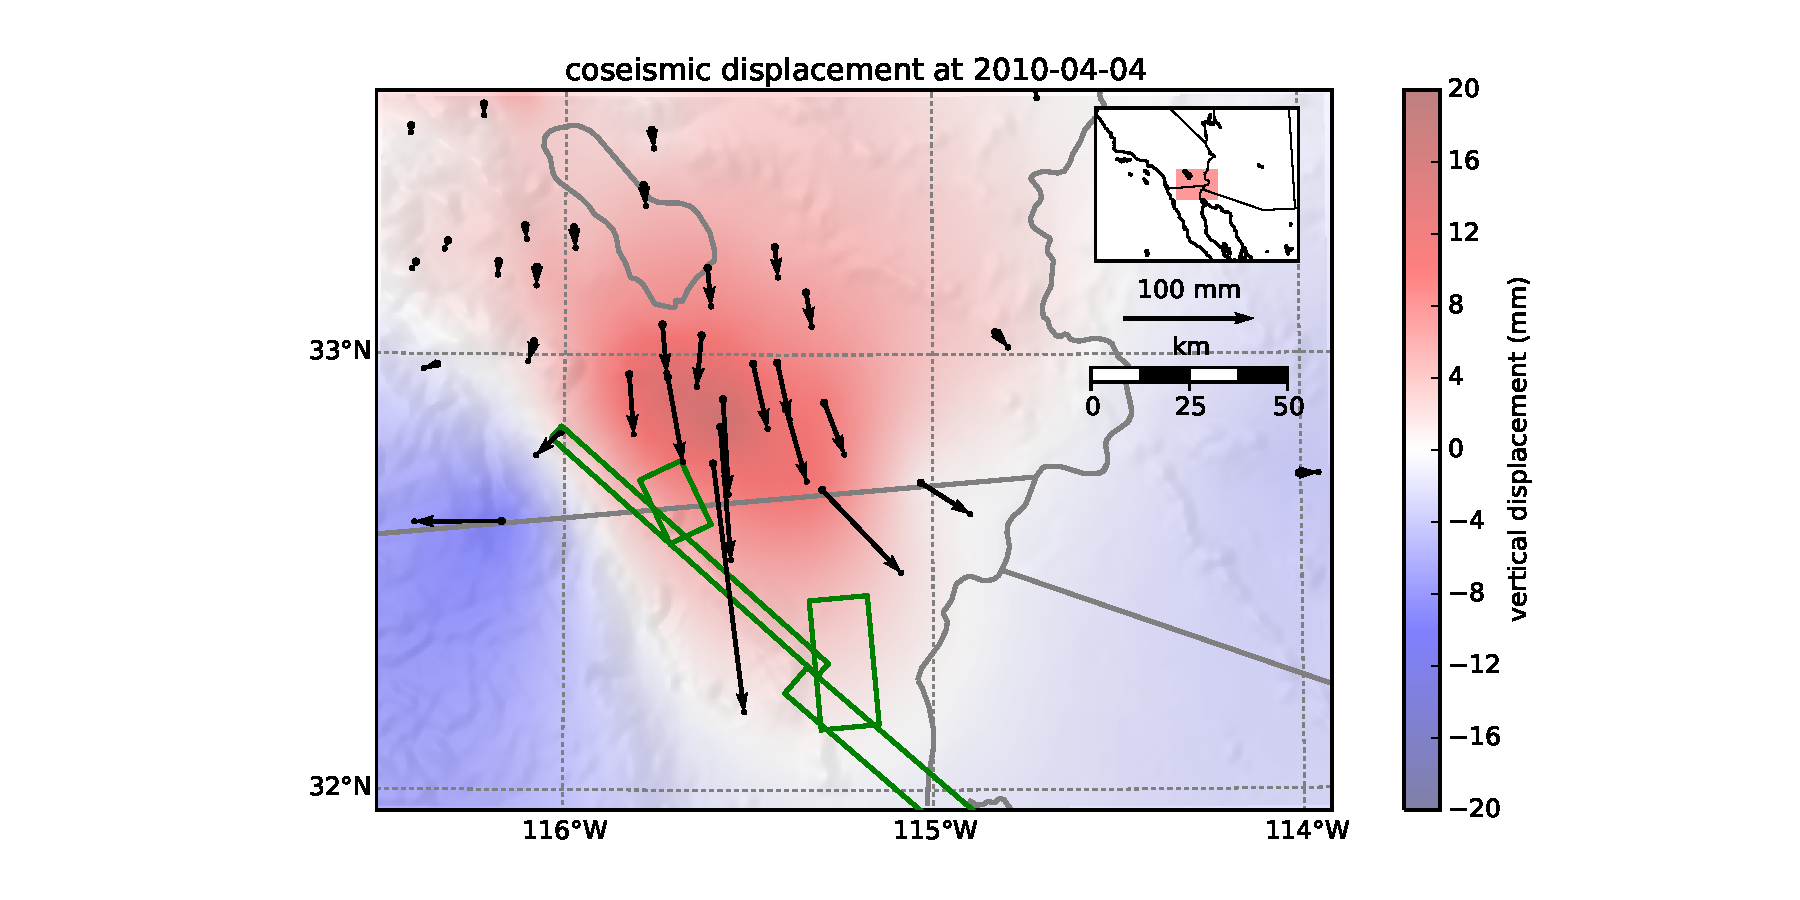
\includegraphics[scale=0.6]{Figures/near_field_data_1}
\centering 
\caption{near field coseismic}
\label{nearfield1}
\end{figure}

\begin{figure}
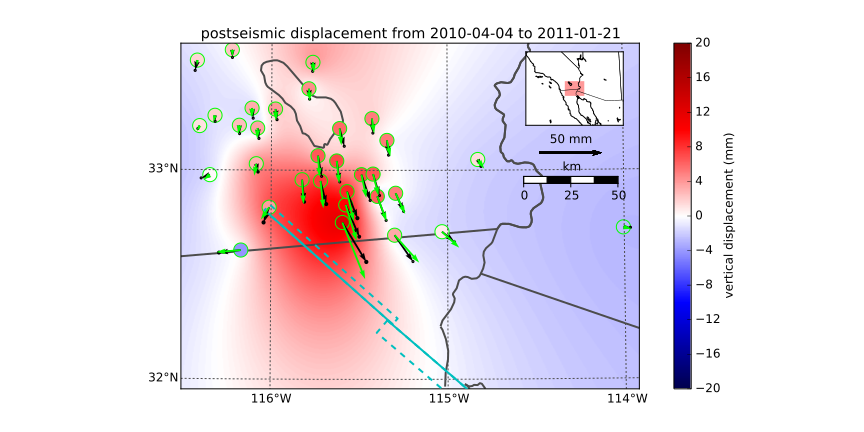
\includegraphics[scale=0.6]{Figures/near_field_data_2}
\centering 
\caption{near field coseismic}
\label{nearfield2}
\end{figure}

\begin{figure}
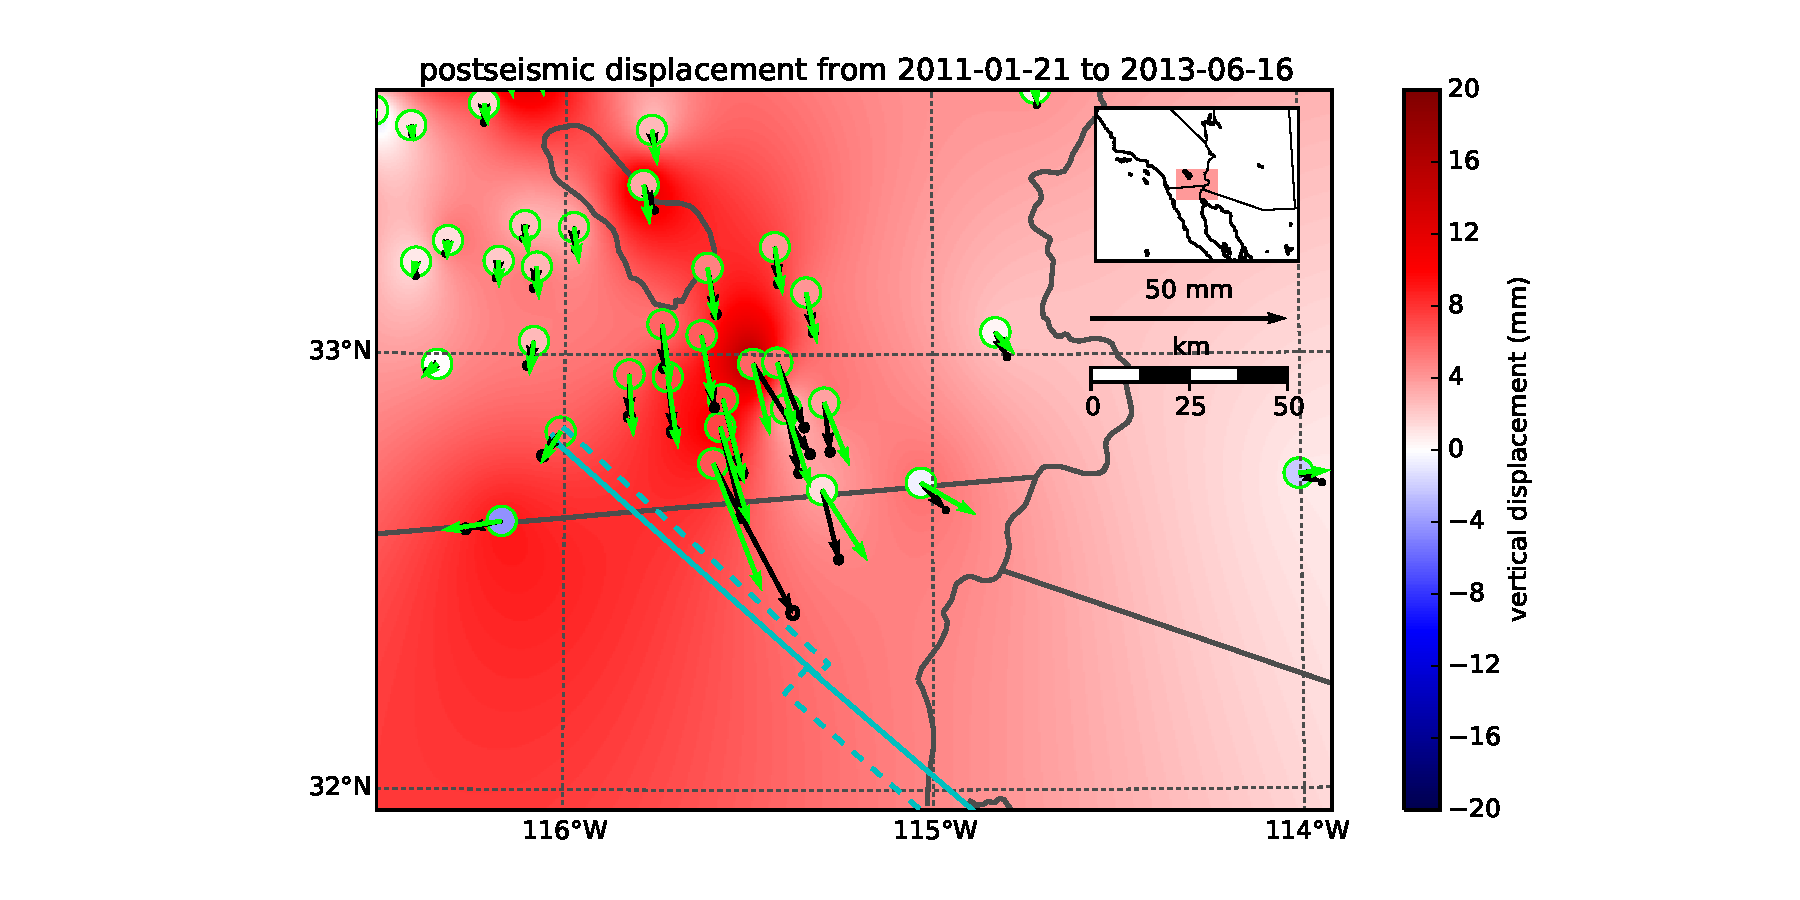
\includegraphics[scale=0.6]{Figures/near_field_data_3}
\centering 
\caption{near field coseismic}
\label{nearfield3}
\end{figure}

\begin{figure}
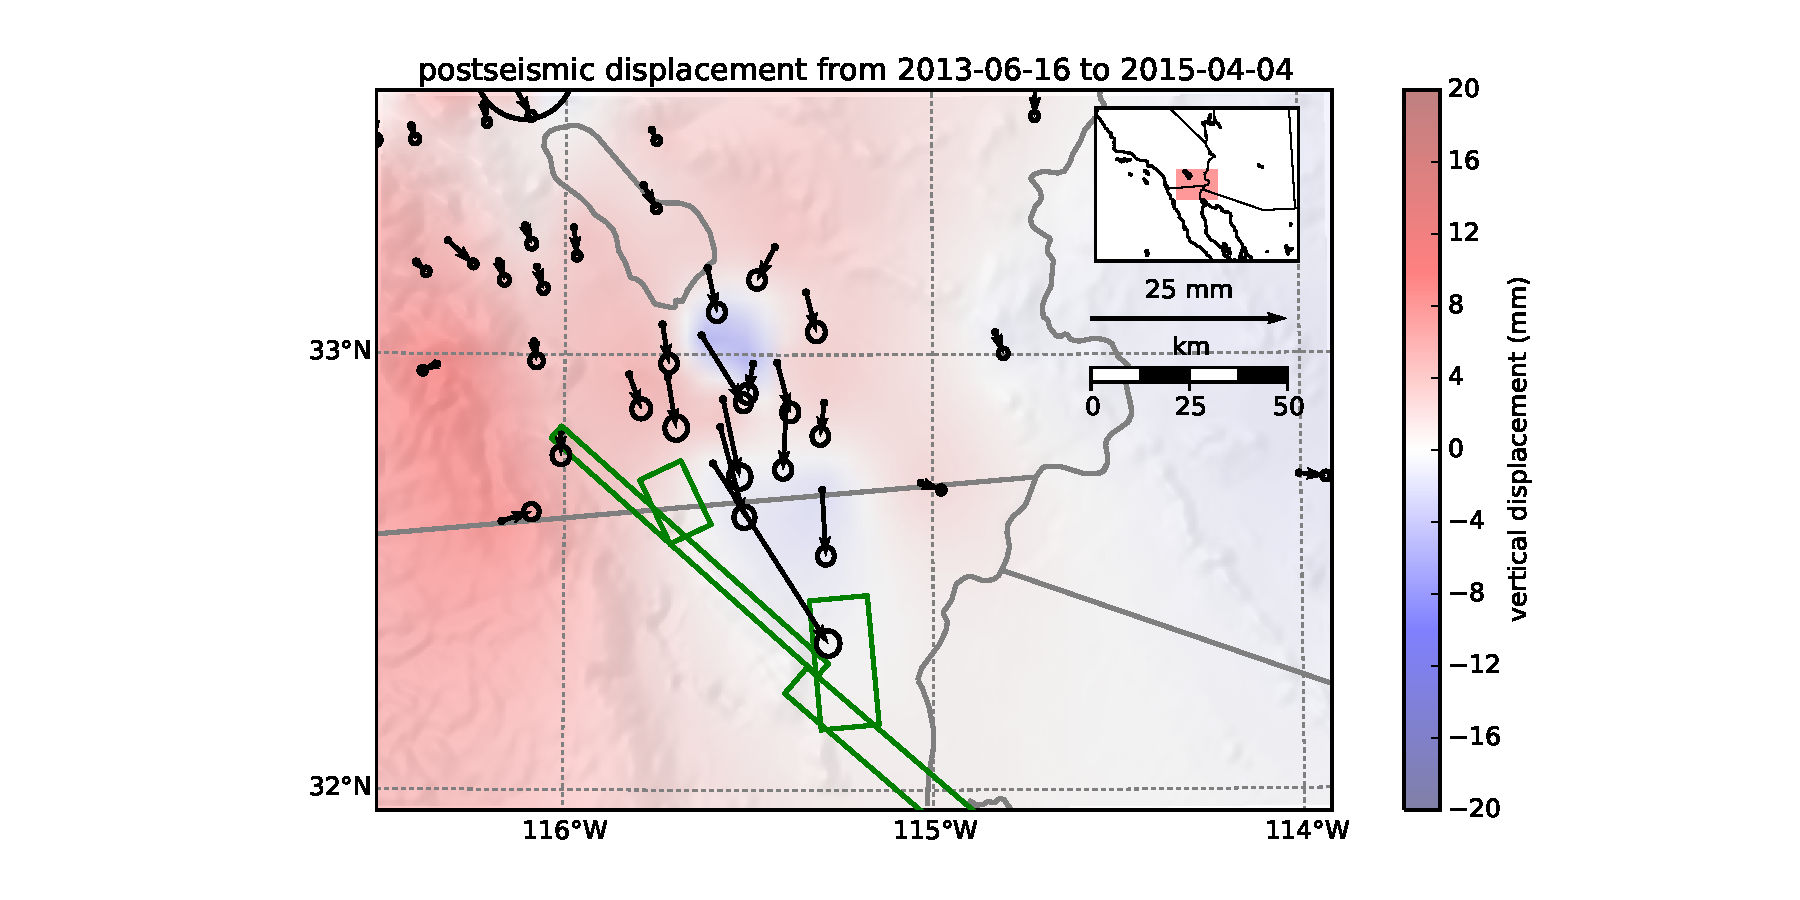
\includegraphics[scale=0.6]{Figures/near_field_data_4}
\centering 
\caption{near field coseismic}
\label{nearfield4}
\end{figure}

\begin{figure}
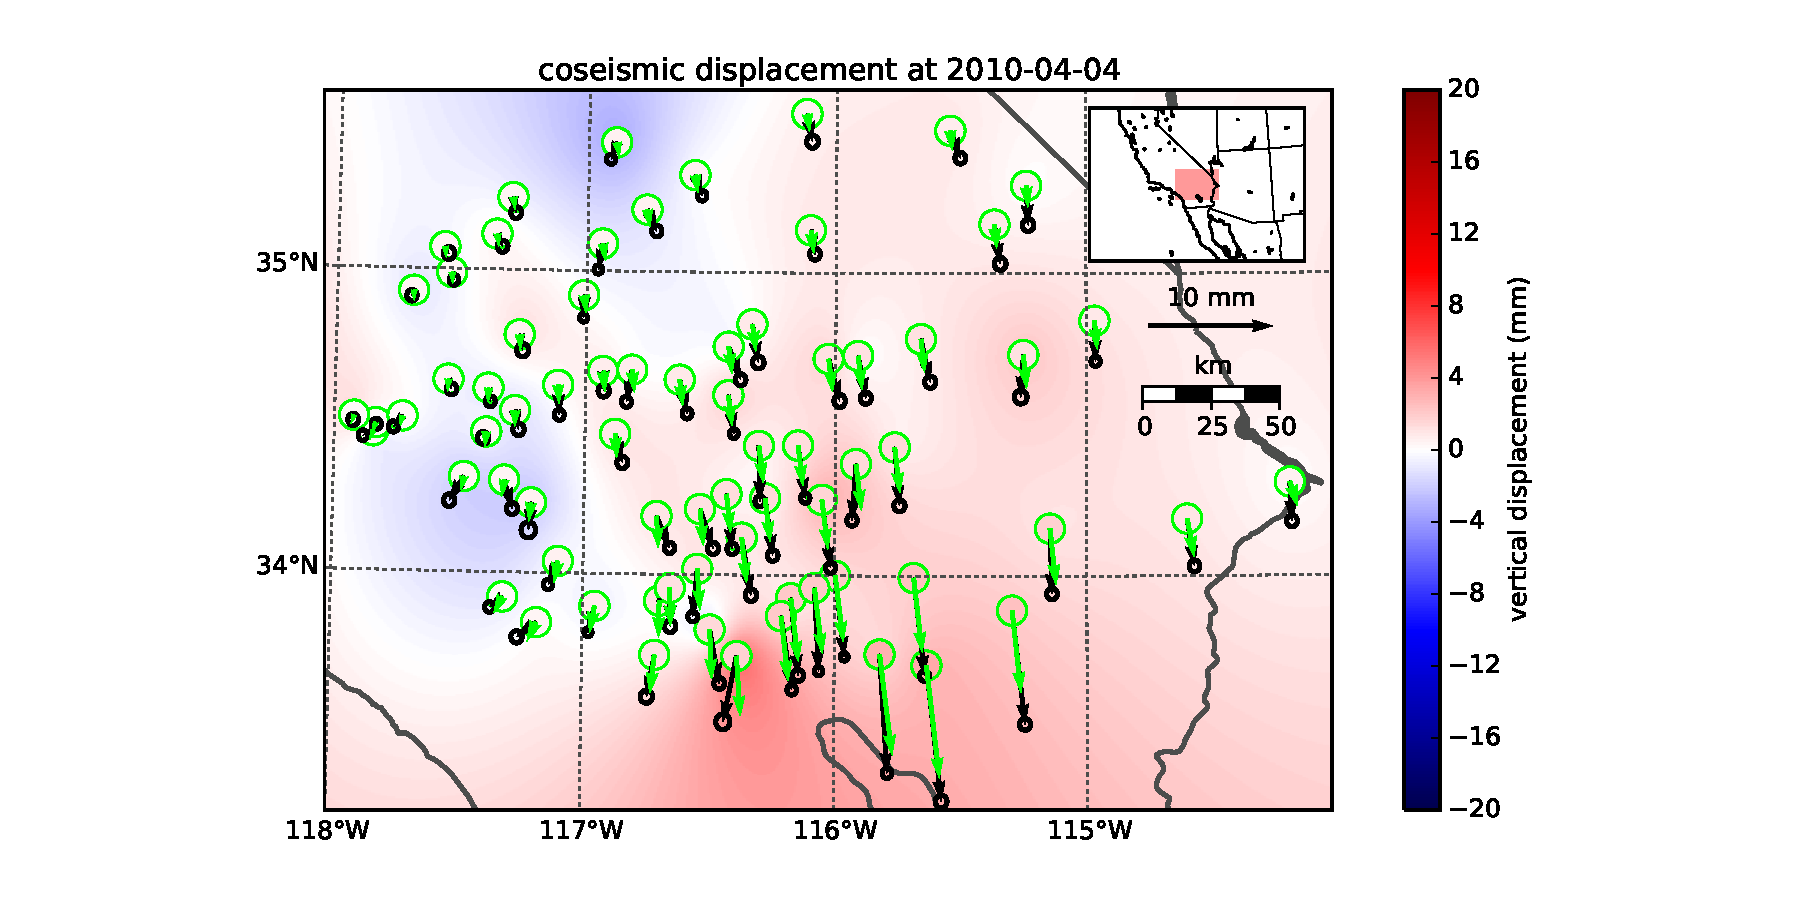
\includegraphics[scale=0.6]{Figures/far_field_data_1}
\centering 
\caption{near field coseismic}
\label{farfield1}
\end{figure}

\begin{figure}
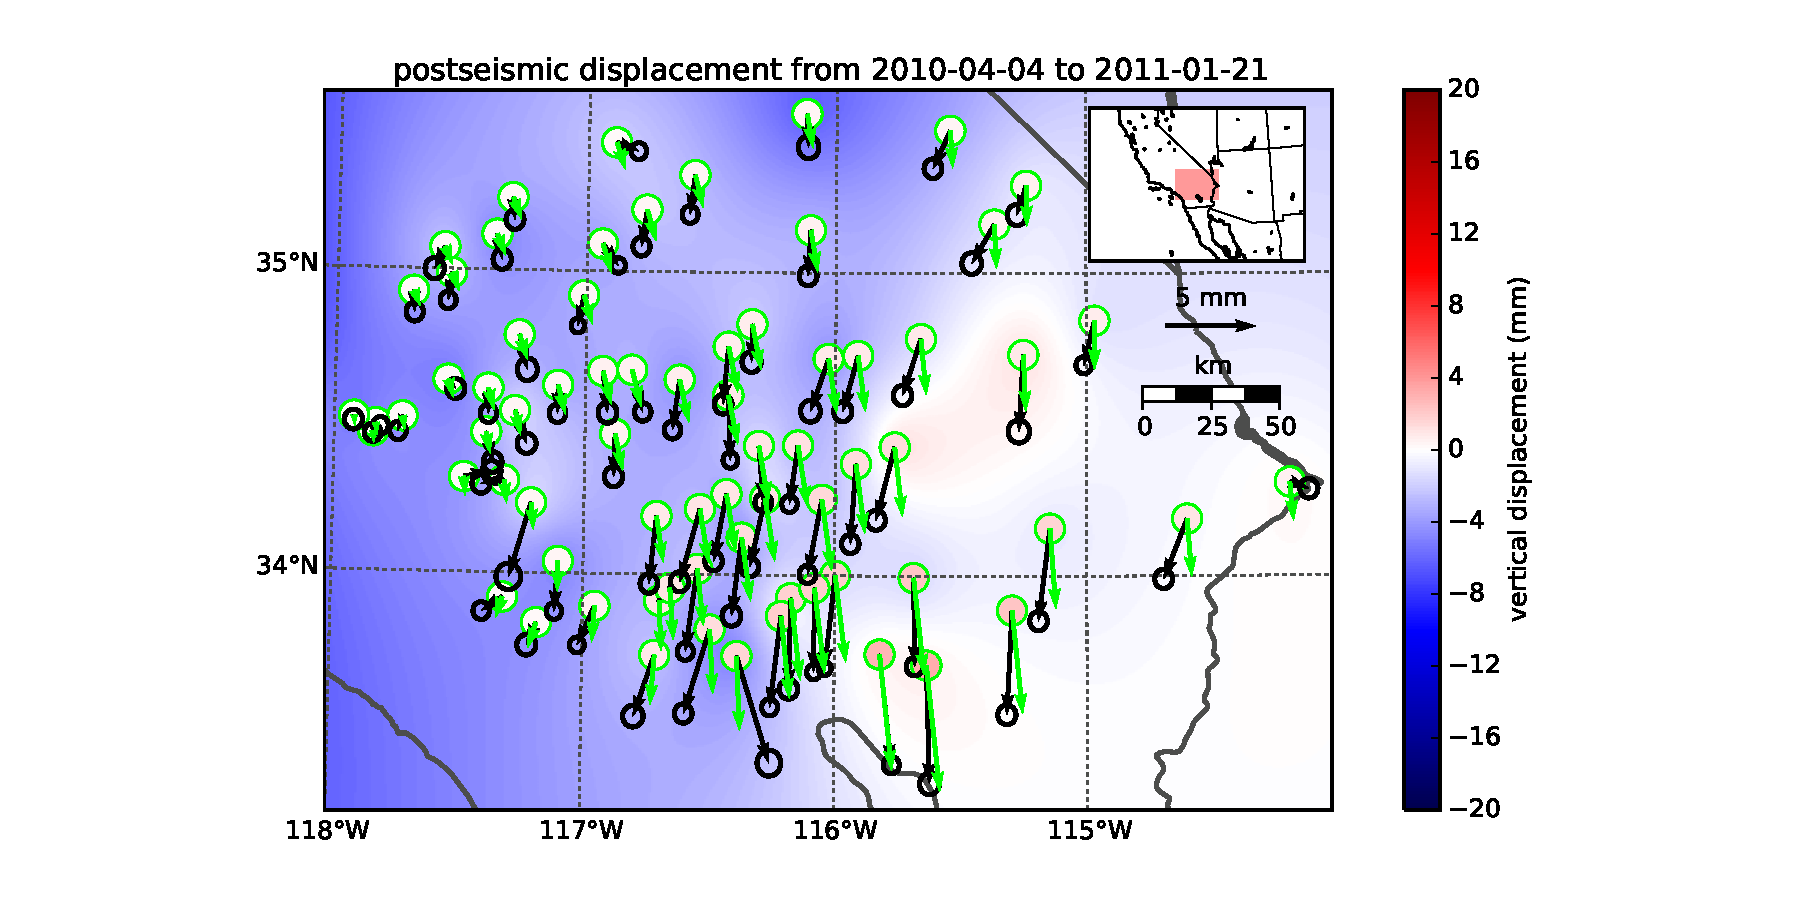
\includegraphics[scale=0.6]{Figures/far_field_data_2}
\centering 
\caption{near field coseismic}
\label{farfield2}
\end{figure}

\begin{figure}
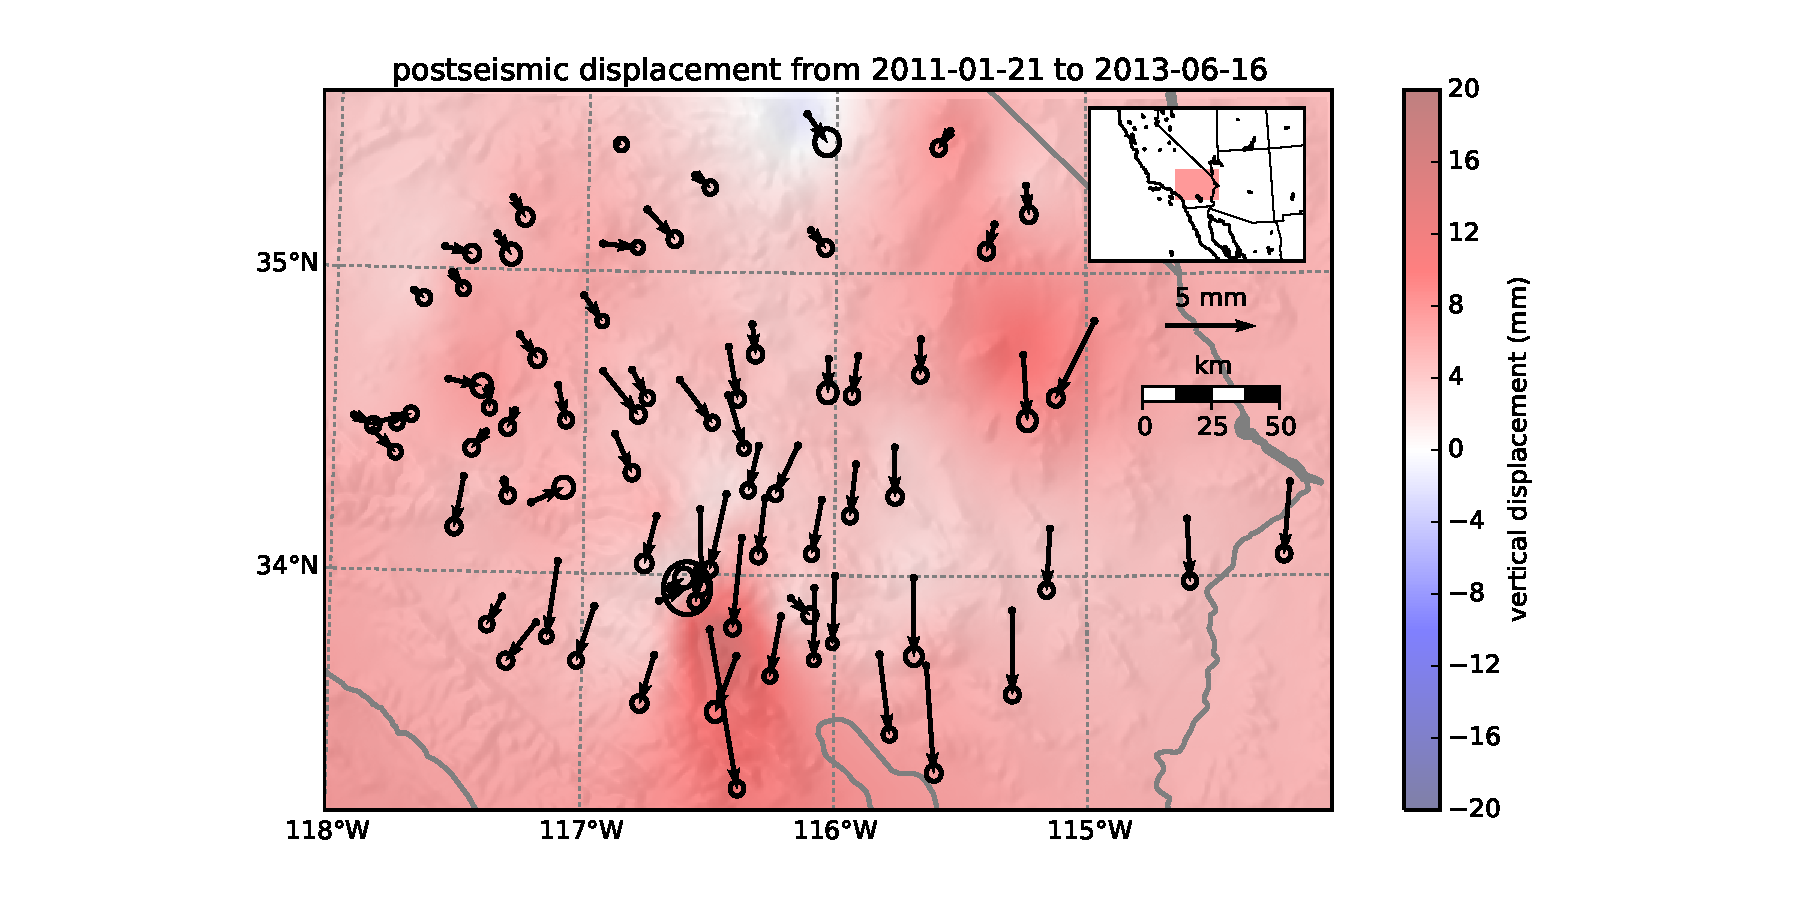
\includegraphics[scale=0.6]{Figures/far_field_data_3}
\centering 
\caption{near field coseismic}
\label{farfield3}
\end{figure}

\begin{figure}
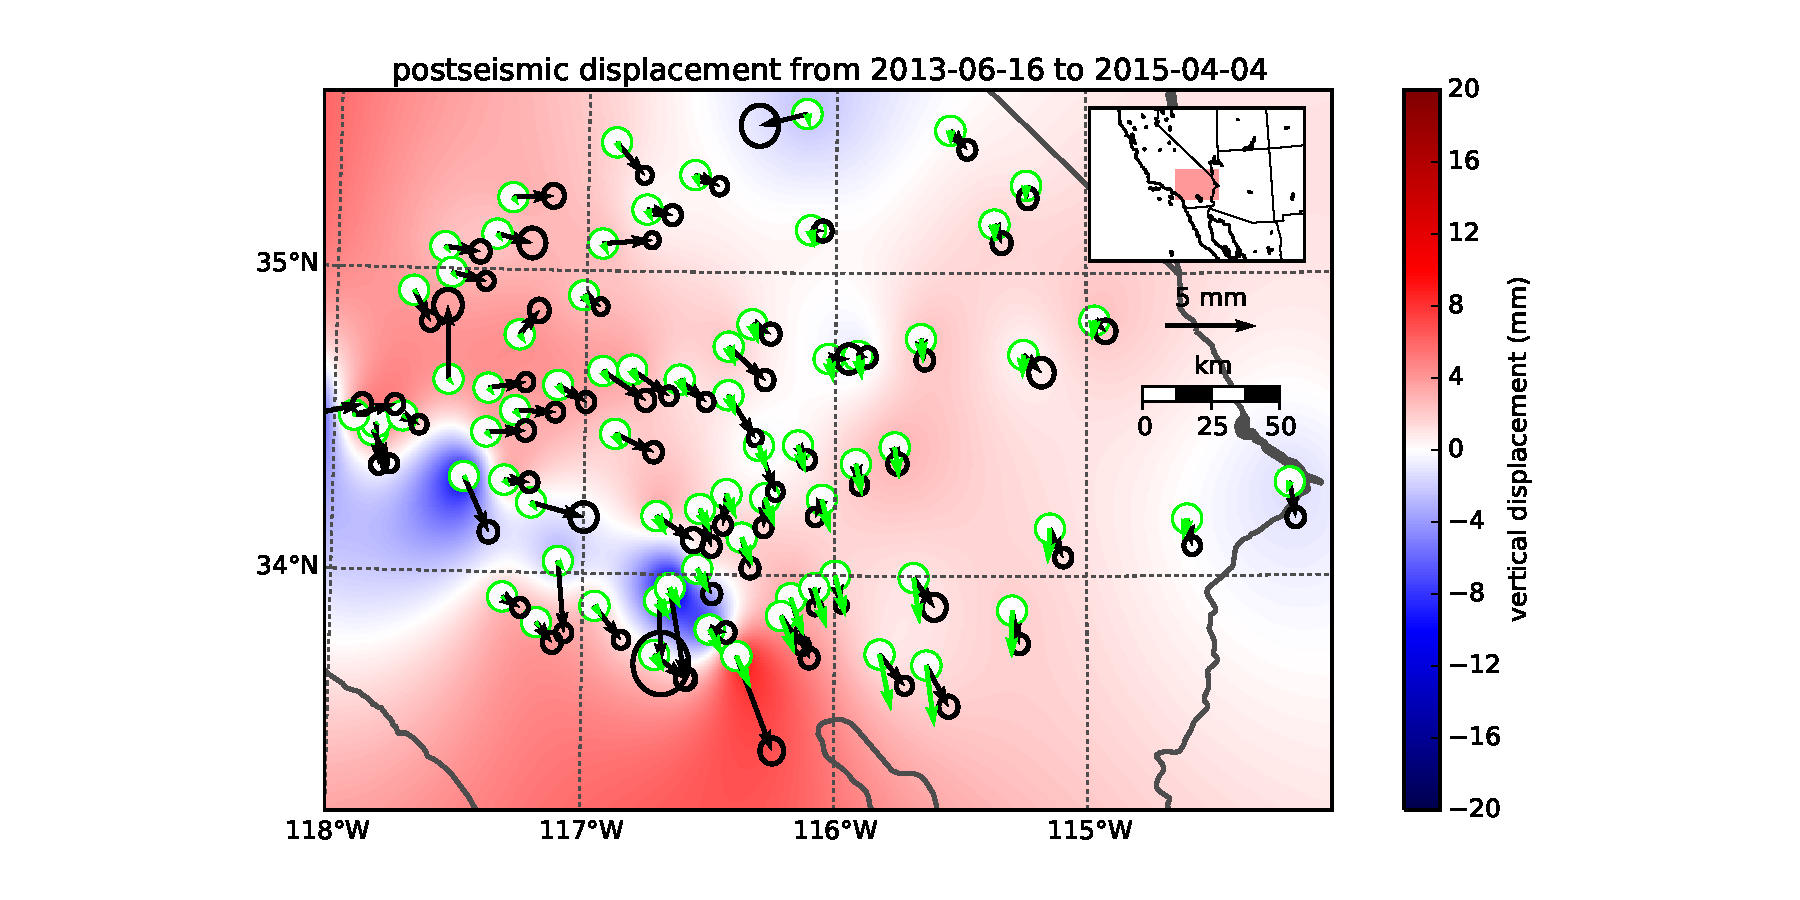
\includegraphics[scale=0.6]{Figures/far_field_data_4}
\centering 
\caption{near field coseismic}
\label{farfield4}
\end{figure}

We show the difference in $u(t)$ for each station from 0 to 0.8 years (figure \ref{nearfield2} and \ref{farfield2}), 0.8 to 3.2 years (figure \ref{nearfield3} and \ref{farfield3}), and from 3.2 to 5.0 years (figure \ref{nearfield4} and \ref{farfield4}).  For far field stations (figure \ref{farfield2}, \ref{farfield3}, and \ref{farfield4}), we can see a clear south trending displacement throughout the first 3.2 years in stations as far as 400 km from of the El Mayor Cucapah epicenter.  These displacements are most pronounced along the direction of the El Mayor-Cucapah P and S axis, as would be expected for postseismic deformation.  Beyond 3.2 years, The southward trending far field postseismic deformation is barely perceptible. There is however, an eastward trend in far field stations just west of the Hector Mine epicenter.  We suspect this this deformation, which is inconsistent with the pattern expected for El Mayor-Postseismic, is the result of continued transient postseismic deformation following the Hector Mine earthquake.  The vertical deformation in the far field is difficult to attribute to postseismic processes.  Most far field stations display an initial subsidence for the first year after the El Mayor-Cucapah earthquake followed by continued uplift.  This trend in vertical deformation can be observed in all three of the quadrants where postseismic data is available, which means that the vertical deformation does not exhibit an anti-symetric quadrant pattern, as would be expected for postseismic processes.  Although we use vertical deformation in our subsequent analysis, we do not put an emphasis on trying to describe the vertical deformation as it likely has non-tectonic origins.        

Near field deformation is show in figures \ref{nearfield2}, \ref{nearfield3}, and \ref{nearfield4}.  The near field deformation is notably sustained when compared to the far field deformation.  Namely, the station in this study which is closest to the El Mayor-Cucapah epicenter, P496, is moving at a steady rate of ~1.4 cm/yr to the south five years after the El Mayor-Cucapah earthquake.  Vertical postseismic deformation in the near field does display a quadrant pattern which is consistent with the coseismic vertical deformation, suggesting that it is indeed resulting from tectonic processes.  However, the vertical postseismic deformation signal is only apparent in the early postseismic period (figure \ref{nearfield2}).  As with the far field deformation, there is a general trend of uplift in the near field one year after the earthquake which we do not consider to be related to postseismic processes.  

\section*{Postseismic Modeling}

outline:

-dismiss poroelastic rebound

-Discuss justification of afterslip as a mechanism
 -vertical deformation argument
 -Kayla's paper and Haukson
 -discuss fault geometry
 
-Discuss viscoelastic relaxation
  - discuss rheologic models and parameters needed to estimate

-Discuss approximation, implications for all rheologic models
-discretization of the lithosphere
-discuss the nitty gritty inverse method

- issue with nonuniqueness of deep afterslip and crustal flow

-discuss fault geometry and modeling assumptions. including elastic properties. and Kayla's paper

-Discuss discretization of slip and viscosity

-discuss early postseismic approximation

In this paper, we seek to find the mechanisms driving five years of postseismic deformation following the El Mayor-Cucapah earthquake. We consider afterslip and viscoelastic relaxation in the lithosphere and/or asthenosphere as candidate mechanisms.  Poroelastic rebound has also been used to model postseismic deformation (cite); however, \cite{Gonzalez-ortega2014} suggest that any contribution to postseismic deformation from poroelastic rebound would be negligable.  Additionally, we are considering stations which are sufficiently far away from the main rupture that poroelastic rebound should be insignificant.  

In this study we estimate coseismic and time dependent postseismic fault slip, both of which are assumed to occur on the fault geometry estimated by \cite{Wei2011a} with some modifications.  Field studies \cite{Fletcher2014} and LIDAR observations \cite{Oskin2012} have revealed a significantly more complicated fault geometry than what was inferred by \cite{Wei2011a}, especially within the Sierra Cucapah.  However, we find the relatively simple coseismic fault geometry from \cite{Wei2011a} to be sufficient because most of the stations used in this station are sufficiently far from the El Mayor-Cucapah epicenter that they are insensitive to the details in the fault geometry found by \cite{Fletcher2014} and \cite{Oskin2012}.  We do, however, modify the fault geometry from \cite{Wei2011a} by extending segment 2 northward by 40 km which is motivated by the clustering of aftershocks on the northern tip of coseismic rupture zone \cite{Kroll2013} \cite{Hauksson2011}.  This extended fault segment was also found to be necessary by \cite{Rollins2015} and \cite{Pollitz2012} for describing postseismic deformation.     

We consider a variety of rheologic models for the lithosphere and asthenosphere in this study.  The simplest rheologic model would be to consider the lithospere and asthenosphere to be effectively elastic. In such case, the rheologic parameters, consisting of the Lame parameters, $\lambda$ and $\mu$, and density, $\rho$, are reasonably well known, leaving the only unknowns to be the distribution of fault slip, which can be easily estimated due to the linearity of the forward problem. \cite{Rollins2015} found that postseismic deformation following the El Mayor-Cucapah earthquake can be well explained with afterslip on the coseismicly ruptured fault, which has been extended down to the lithosphere-asthenosphere boundary inferred by \cite{Lekic2011}, and they did not require any viscoelastic relaxation to describe the observations.  They did however, find that the amount of afterslip required for the southernmost fault segment to be unrealistically large, equivalent to a Mw7.2 earthquake.  Since most of the GPS data is located north of the rupture zone, slip on the Indiviso fault segment is least constrained and could be acting as a proxy for distributed relaxation in the lower crust or upper mantle. 

It is well understood that afterslip at sufficiently great depths can explain postseismic deformation resulting from viscoelastic relaxation \cite{Savage1990}, and so in the interest of preventing a non-unique solution, we assuming afterslip to occur only at seismogenic depths (<15 km), and allow for viscoelastic relaxation in the lower crust (15-30 km) depth and the upper mantle.We choose such shallow constraints on afterslip because rate-state friction based models would suggest afterslip to occur at shallow depths to accommodate a coseismic slip deficit \cite{Marone1991}, which is indeed inferred in the coseismic models by \cite{Wei2011a} and (Fialko 2010). Additionally, as noted by \cite{Rollins2015} the postseismic uplift just north of the rupture zone can be well described with slip at seismogenic depths, while afterslip which is constrained to depths beneath 15 km predicts subsidence in that region.  

A third reason for constraining slip to be shallower than 15 km depth is because we seek to estimate a lower crustal viscosity and trying to simultaneously estimate deep afterslip and a lower crustal viscosity leads creates a significant null space.  The reason for this is because viscoelastic relaxation within the lower crust of resulting from slip that is also within the lower crust will produce surface deformation in the direction opposite of slip. That is to say, the predicted viscoelastic deformation will cancel out the elastic deformation resulting in a trade off where a viscoelastic relaxation within a weak lower crust can be canceled out by slip at lower crustal depths.      

With afterslip constrained to shallow depths, we must now select a viscoelastic rheology for the lower crust and upper mantle. Maxwell viscoelasticity, which can be schematically illustrated as a spring and dashpot connected in series, is the simplest and commonly used rheologic model for studies on postseismic deformation NUR IS SLS! (e.g. \cite{Nur1974}, \cite{Pollitz2000}, \cite{Hetland2003},\cite{Freed2006a}, \cite{Johnson2009}, \cite{Hearn2009}).  Assuming Maxwell viscoelasticity introduces a single the unknown rheologic parameter. A Maxwell viscoelastic model of the lithosphere would predict deformation that decays steadily over time, which fails to describe the multiple timescales of relaxation observed in postseismic deformation \cite{Savage1997}.  An additional deficiency in modeling the lithosphere with a Maxwell rheology is that inferred viscosities tend to depend on the the timescale of the geophysical process being modelled \cite{Peltier1981}. When assuming Maxwell viscoselasticity, upper mantle viscosities for Southern California inferred from postseismic deformation tend to be on the order of $10^{18}$ Pa s (\cite{Pollitz2000}, \cite{Thatcher2008}, \cite{Spinler2015}. However, studies of interseismic deformation \cite{Lundgren2009} and lake loading \cite{Luttrell2007}, which are both processes that occur on the timescale of $~10^2$ years, infer a Maxwell viscoelastic upper mantle with a viscosity on the order of $10^{19}$ Pa s.  

To account for the apparently multiple timescales of relaxation, \cite{Pollitz2003} used a Burgers rheology upper mantle to model postseismic deformation following the Hector Mine earthquake and inferred a transient viscosity of $1.6\times10^{17}$ Pa s and a steady state viscosity of $4.6\times10^{18}$ Pa s, which still falls short of the steady state viscosity required for longer term geophysical processes. The particularly weak transient viscosity was found to be necessary to describe the early rapid postseismic deformation, although other researchers have successfully described the early postseismic deformation for the same earthquake with fault creep and poroelastic rebound. Nevertheless, laboratory experiments have demonstrated that mantle rock exhibits two phases of relaxation which can be adequately described with a Burgers rheology \cite{Chopra1997} and we should expect to see some postseismic signal resulting from transience viscoelasticity. 

The third linear viscoelastic rheology which we consider is the Zener model, often referred to as a standard linear solid, whose mechanical analogue consists of a spring connected in series with a Kelvin element. A generalization of the Zener model, consisting of a series of Kelvin elements connected in series each of which representing a distinct deformation mechanism, is commonly used to describe the spectrum of frequency dependent attenuation \cite{Liu1976}.  The highest viscosity needed to describe attenuation of earth's lowest frequency normal modes is on the order of $10^{16}$ Pa s \cite{Yuen1982}, which is too weak to be perceptible in the GPS data used in the present study.  

As an exploratory step, we also perform a slip inversion, assuming an elastic lithosphere and asthenosphere.  The difference between the analysis in  \cite{Rollins2015} and the present study is that we include a wider range of GPS stations in our inversion and we also perform a temporal estimation of afterslip, as opposed to estimating slip at a single epoch. The material properties used in our inversion are given in table 1 and are consistent with the properties used by \cite{Wei2011a} and the 1D SCEC background velocity model.  We discretize the          

 and the constrained and the only para.  where the rheologic parameters       
In order to model postseismic deformation we must ddetermine an appropriate rheologic model for the lithosphere and asthenosphere.  
To model postseismic deformation we must first assume a rheologic model.  The simplest viscoelastic rheologic model would be a Maxwell model, where shear stresses and strains can be described with the mechanical analogy of a spring and dashpot connected in series.  If coseismic and postseismic slip, described by $s(\xi,t)$, occurs on a fault $F$, and viscoelastic relaxation of subsequent stresses occurs in a Maxwell viscoelastic medium $L$, which has a spatially variable viscosity, $\eta(\zeta)$, then coseismic and postseismic deformation can be described by 
\begin{equation}\label{GeneralForward}
  u(x,t) = \int_F s(\xi,t)g(x,\xi)d\xi + 
           \int_0^t\int_F s(\tau,\xi) f(t-\tau,x,\xi) d\xi d\tau
\end{equation}
where $g(x,\xi)$ is the elastic Green's function relating slip at $\xi$ to instantaneous displacement at $x$ and $f(t,x,\xi)$ describes the rate of deformation at $x$ and time $t$ resulting from viscoelastic relaxation of stresses induced by slip  at $\xi$.  The variables which we are primarily concerned with estimating in this study are $s(\xi,t)$ and $\eta(\zeta)$.  Numerous experimental and geophysical studies suggest that a Maxwell rheology is inappropriate to describe the behaviour of the uppermost mantle \cite{Chopra1997} \cite{Pollitz2003} \cite{Freed2004} and so we do not limit ourselves to exploring Maxwell viscolesticity.  When considering other stress-linear viscoelastic models, such as a Zener or Burgers model, the description of displacements remains unchanged from eq \ref{GeneralForward} except that $f$ is parameterized by additional rheologic parameters which must also be estimated.  The difficulty in  determining an appropriate rheologic model and then estimating $s(\xi,t)$ and the unkown rheologic parameters from observations of $u(x,t)$ is that it is a nonlinear inverse problem with many unknown parameters and a computationally expensive forward problem.  We can greatly simplify the inverse problem by first considering the early postseismic period where we can approximate $u(x,t)$ for any stress-linear viscoelastic rheology as
\begin{equation}\label{ApproxForward}
  u(x,t) = \int_F s(\xi,t)g(x,\xi)d\xi + 
           \int_0^t\int_F\int_L \frac{s(\tau,\xi)}{\eta_\mathrm{eff}(\zeta)} h(x,\xi,\zeta) d\zeta d\xi d\tau
\end{equation}

what this gives us is a prior constraint on lithospheric viscosity initial that is unbiased by neglecting the contribution of afterslip! 


It can be shown (\cite{Hines2015}),     

other rheologic models in this study      viscoelasticity is We also test rheologic models other than viscoelasticity to describe    




There are numerous other parameters which are not known, but will be considered known in this study.   


   Inherent in f is also a stress-linear viscoelastic model.   In this study we will be be known while try to consider             

    

   The early near field postseismic vertical deformation does show a quadrant pattern and is also consistent with the coseismic vertical deformation.  Given         

that would not becomes there is no longer a coherent far field deformation signal. This is in contrast to near field displacements which persists for the entire 5.0 years of data used in this study. Figure () further illustrates the difference in deformation regimes between near field and far field station.  



We use a fault geometry from \cite{Wei2011}, which was determined using teleseismic, GPS, and InSAR data.  

After the El Mayor-Cucapah earthquake, additional GPS stations were installed In Baja California to record postseismic deformation with better spatial coverage.  Two of the stations PTAX and PHJX were installed near the epicenter in the Cucapah Mountains.  We do not include these two stations in our analysis because the geometry of the faults that ruptured during the earthquake is more complicated than our assumed fault geometry \cite{Oskin2012} \cite{Fletcher2014} and the near field stations would be most sensitive to error in our geometry. We also leave of these near field stations in order to avoid any near field processes which we do not consider in this paper \cite{Gonzalez-ortega2014}. Numerous stations exhibit extraneous signals which can be 

\section*{Rheological constraints}

\section*{Results}
\section*{Acknowledgements}

This material is based on EarthScope Plate Boundary Observatory data services provided by UNAVCO through the GAGE Facility with support from the National Science Foundation (NSF) and National Aeronautics and Space Administration (NASA) under NSF Cooperative Agreement No. EAR-1261833.

\bibliographystyle{apalike}
\bibliography{mybib}

\end{document}

